\documentclass[onecolumn,preprintnumbers,amsmath,amssymb]{revtex4}

\usepackage{graphicx}
\usepackage{dcolumn}
\usepackage{bm}
\usepackage{epsfig}
\usepackage{amssymb}
\usepackage{amsmath}
%\usepackage{epspdfconversion}

\newcommand{\lsim}{\mathrel{\hbox{\rlap{\lower.55ex\hbox{$\sim$}} \kern-.3em \raise.4ex \hbox{$<$}}}}
\newcommand{\gsim}{\mathrel{\hbox{\rlap{\lower.55ex\hbox{$\sim$}} \kern-.3em \raise.4ex \hbox{$>$}}}}
\newcommand{\beq}{\begin{equation}}
\newcommand{\eeq}{\end{equation}}
\newcommand{\beqa}{\begin{eqnarray}}
\newcommand{\eeqa}{\end{eqnarray}}
\newcommand{\drm}{\mathrm{d}}
\newcommand{\grad}{\vec{\nabla}}
\newcommand{\Mpl}{M_\mathrm{Pl}}
\newcommand{\apjs}{ApJ Supp.}
\newcommand{\alphanu}{\alpha_\nu}
\newcommand{\ellnu}{\ell_\nu}
\newcommand{\taunu}{\tau_\nu}
\newcommand{\Inu}{I_\nu}
\newcommand{\bsp}{\begin{split}}
\newcommand{\esp}{\end{split}}
\newcommand{\sigmanu}{\sigma_\nu}
\newcommand{\Snu}{S_\nu}
\newcommand{\vecE}{\vec{E}}
\newcommand{\vecB}{\vec{B}}
\newcommand{\vecA}{\vec{A}}
\newcommand{\vecr}{\vec{r}}
\newcommand{\del}{\partial}
\newcommand{\ceil}[1]{\left\lceil #1 \right\rceil}
\newcommand{\floor}[1]{\left\lfloor #1 \right\rfloor}

\newcommand{\sigv}{\sigma_v}
\newcommand{\rhovir}{\bar{\rho}_\mathrm{vir}}
\newcommand{\mvir}{M_\mathrm{vir}}
\newcommand{\rvir}{R_\mathrm{vir}}
\newcommand{\Om}{\Omega_\mathrm{M}}
\newcommand{\Omo}{\Omega_\mathrm{M0}}
\newcommand{\mearth}{M_\oplus}
\newcommand{\msun}{M_\odot}
\newcommand{\mbd}{m_\mathrm{bd}}
\newcommand{\thetaEiso}{\theta_E^\mathrm{iso}}



\begin{document}
 
\title{Aligning the Stars - Aurora Localization via Star Trails}
\author{ Laura Culp, Fangda Li, Andre Recnik}

\begin{abstract}
This is a brief description of the analytical and numerical methods used to solve the "Aligning the Stars" challenge outlined for the NASA SpaceApps Hackathon in Toronto, Ontario.
\end{abstract}

\maketitle

\section{\bf Introduction }

Auroras are visible in many time-lapse picture sequences taken from the International Space Station (ISS).  Our goal is to use this data to determine the the location of the aurora on the earth.  The only additional information available is the location (Nadir point and altitude) of the ISS for each frame.

\section{ \bf Determining Camera Orientation }

Given only the Nadir point of the ISS and its altitude, one can determine circular horizon centred on the ISS in which the visible aurora must be constrained.  However, the camera's field of view covers only $\sim \pi/3$, so the problem becomes the determination of where this field of view wedge is centred.

An exhaustive astrometric search was first implemented and found to be computationally intractable since the search grid spacing in RA, DEC, and frame rotation angle must be much smaller than the inter-stellar spacing on the frame $\ll 1$ degree.  We employ a much more efficient method via star trail mapping to determine the velocity of the stars and thus the angle of the camera off the orbit of the ISS.

\section{\bf Computational Method Outline }

Our method was as follows:
\begin{enumerate}
\item Segment images into 'earth' and 'sky' using k-means
\item Extract the brightest stars from each frame
\item Stack extracted stars to form star-trails
\item Calculate the length of each star-trail and convert to velocity data
\item Determine the angular offset of the camera from the ISS orbit
\end{enumerate}

Once the orientation of the camera relative to the International Space Station has been determined, the approximate location of the aurora in each image is placed on a map using the following method:
\begin{enumerate}
\item Approximate where the aurora is in the image via segmentation
\item Calculate the area of the earth visible in the image
\item Project the approximate location of the aurora onto the earth
\end{enumerate}

The details of these methods will be explained further below. 

\subsection{ \bf Image Segmentation }

In order to avoid incorrect identification of stars in the images, the area in the image belonging to the earth must be separated from the area in the image belonging to the sky.  The location of the aurora itself must also be approximated in the image in order to be able to map it to a location on the earth.  This can be done using a computer vision technique called segmentation.

There are two methods of image segmentation that were attempted: k-means and level sets.  Each method worked, but the k-means algorithm worked more efficiently and was able to provide a segmentation of both the aurora and the earth at the same time.  These methods are briefly described.

\subsubsection{ \bf k-means }

K-means segmentation is a clustering technique which separates the image into a given number, k, of clusters, each centered around a Gaussian distribution.  There is an efficient implementation of this algorithm included in a library in matlab, 'kmeans'.  This implementation was used.

In order to more-accurately identify the clusters, the entire image was scaled down and blurred.  This avoids anomelies being placed in the incorrect clusters.

\subsubsection{ \bf Level Sets }

The level set method tracks an evolving contour line.  The approximate level sets are tracked, and when the slope of the contour line is greater than a given parameter, the current contour line is used to determine a cut in the image.  This only separates the image into two different sections, and can take slightly longer than the k-means algorithm.  In addition, there are multiple parameters that need to be played with and correctly chosen in order to get the desired results.

An implementation of this method given by Jeff Orchard in a Medical Image Processing course at the University of Waterloo was used. 

\subsection{ \bf Star-Trail Creation }

The star trails are created by first extracting the stars from the segmented images by comparing the median of a 3x3 grid and the median of a 9x9 grid around each pixel.  This extracts just the brightest stars.

Then the extracted stars from each image are added together to form the star trails.  To make the velocity extraction process more robust, the images are not given an equal weights.  The first 5 images are given a small weight, the middle images are given a larger weight, and the last 5 images are given a very large weight.  This allows the velocity extraction process to detect what direction the trail is moving in, and if the trail is complete (contains both a start and end point). 

\subsection{ \bf Velocity Extraction }

To extract the velocity from the star trails we simply need to measure the star trail lengths, and divide by the time interval. 

To do this we look at every pixel in the image, and when we find a part of a star trail we use a flood fill algorithm to expand the area to the full trail.  Given this full trail, we can compute the minimum and maximum points, and measure the distance between them to get the approximate arc-length.  

Since we changed the weight of the star values for the start and end of the trail, it is possible to check what the direction of the star trail is in.  This also solves the problem of incomplete star trails, were the star exits or enters the frame, since such a trail will lack either a start or end point, or both. 

\subsection{ \bf Camera Orientation Calculations }

Let $p$ be the pixel size and let $f$ be the focal length of the lens.  We define a virtual celestial sphere whose rotation axis is define by the ISS revolution axis.  Given the size of the image frame $2x0 \times 2y0$ pixels and the virtual declination of the centre of the frame and the frame rotation angle $(d0, \theta)$, we then have the tangent plane projection relations for the virtual right ascension $a$ and declination $d$ of a pixel (x, y) in the frame:

\beq
d = \text{Arcsin}\left[\frac{\text{Sin}(d0)+\frac{p \text{cos}(d0)
   (-x+x0+(y-y0) \text{cot}(\theta)) \text{Sin}(\theta)}{f}}{\sqrt{1+\frac{p^2
   (-x+x0+(y-y0) \text{cot}(\theta))^2 \text{Sin}(\theta)^2}{f^2}+\frac{p^2
   ((x-x0) \text{cos}(\theta)+(y-y0) \text{Sin}(\theta))^2}{f^2}}}\right],
\eeq

\beq
a = \text{ArcTan}\left[\frac{p ((x-x0) \text{cos}(\theta)+(y-y0)
   \text{Sin}(\theta))}{f \left(\text{cos}(d0)-\frac{p (-x+x0+(y-y0)
   \text{cot}(\theta)) \text{Sin}(d0) \text{Sin}(\theta)}{f}\right)}\right].
\eeq
where we define the centre of the image to have right ascension $a = 0$.   $d0$ is the angular difference between the direction in which centre of the frame is pointed, and the direction of motion of the ISS.  We analytically extend the above functions to extend their region of applicability over the polar regions of the virtual sphere where they are otherwise singular.
Defining

\beq
\begin{split}
&K(d0, \theta, x, y) \equiv \\
&(f \text{cos}(d0)+p \text{sin}(d0) ((-y+y0) \text{cos}(\theta )+(x-x0) \text{sin}(\theta )))^2 \left(1+\frac{p^2 ((x-x0) \text{cos}(\theta )+(y-y0) \text{sin}(\theta ))^2}{(f \text{cos}(d0)+p \text{sin}(d0) ((-y+y0) \text{cos}(\theta )+(x-x0) \text{sin}(\theta )))^2}\right)
\end{split}
\eeq

\beq
\begin{split}
&J(d0, \theta, x, y) \equiv \\
&f^3 \left(\frac{f^2+p^2 \left(x^2-2 x x0+x0^2+(y-y0)^2\right)}{f^2}\right)^{3/2} \left(1-\frac{(f \text{sin}(d0)+p \text{cos}(d0) ((y-y0) \text{cos}(\theta )+(-x+x0) \text{sin}(\theta )))^2}{f^2+p^2 \left(x^2-2 x x0+x0^2+(y-y0)^2\right)}\right)^{1/2},
\end{split}
\eeq
we differentiate the tangent plane projections with respect to $x$ and $y$, obtaining

\beq
\frac{\partial a}{\partial x}(d0, \theta, x, y) = \frac{p}{K(d0, \theta, x, y)} (-f \text{cos}(d0) \text{cos}(\theta )+p (y-y0) \text{sin}(d0))
\eeq

\beq
\frac{\partial a}{\partial y}(d0, \theta, x, y) = -\frac{p}{K(d0, \theta, x, y)} (p (x-x0) \text{sin}(d0)+f \text{cos}(d0) \text{sin}(\theta ))
\eeq

\beq
\frac{\partial d}{\partial x}(d0, \theta, x, y) = -\frac{p}{J(d0, \theta, x, y)} \left(f p (x-x0) \text{sin}(d0)+\text{cos}(d0) \left(p^2 (x-x0) (y-y0) \text{cos}(\theta )+\left(f^2+p^2 (y-y0)^2\right) \text{sin}(\theta )\right)\right)
\eeq

\beq
\frac{\partial d}{\partial y}(d0, \theta, x, y) = \frac{p}{J(d0, \theta, x, y)} \left(f p (-y+y0) \text{sin}(d0)+\text{cos}(d0) \left(\left(f^2+p^2 (x-x0)^2\right) \text{cos}(\theta )+p^2 (x-x0) (y-y0) \text{sin}(\theta )\right)\right).
\eeq
The revolution of the ISS around the Earth only changes the virtual right ascension of stars in the image and not their virtual declination.  Thus, given a star trail length $(\Delta x, \Delta y)$ over some time $\Delta t$ centred on $(x_c, y_c)$, the residual for a single data point is:

\beq
R(d0, \theta, x_c, y_c) = \left(\Delta x \frac{\partial a}{\partial x}(d0, \theta, x_c, y_c) +\Delta y \frac{\partial a}{\partial y}(d0, \theta, x_c, y_c) - \Delta t\frac{2 Pi}{P}\right)^2 + \left(\Delta x \frac{\partial d}{\partial x}(d0, \theta, x_c, y_c) +\Delta y \frac{\partial d}{\partial y}(d0, \theta, x_c, y_c)\right)^2
\eeq
where P is the period of the ISS revolution.  We minimize the sum of R over all star trails that we extract in the image to optimize the parameters $(d0, \theta)$.

\begin{figure*}
\resizebox{\textwidth}!{
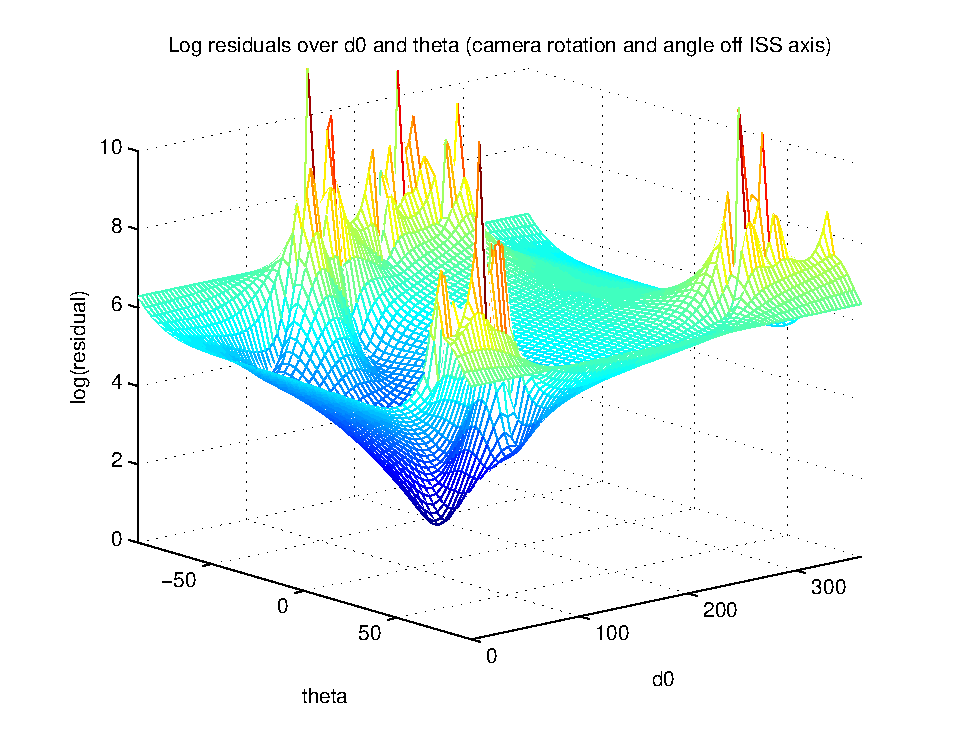
\includegraphics{residuals-1.eps}}
\caption{Summed residual over all data points as a function of camera rotation angle $theta$ (deg) and virtual declination of the frame $d0$ (deg).}
\label{residuals}
\end{figure*}

Note that this procedure does not compute the angle of the camera with respect to the horizon (i.e. how much of the ground vs. sky is shown).  This angle can however be easily computed using the segmentation of the images, and comparing the amount of ground vs. sky in the image. 

\subsection{ \bf Projections and Display of Map }

At this point we have the orientation of the camera, and the approximated aurora and earth segmentation data.  We now need to calculate the area of the earth visible from the camera, and from that, approximate the aurora location.

\subsubsection{ \bf Earth Visible from Camera }

We know the orbit of the ISS. Let the current position of the ISS be $\bf{x}$ and the position of the ISS in the next frame be $\bf{x'}$. We also know the angle of the camera off the axis of the ISS orbit $d0$. 

Since the horizon distance is small compared to the radius of the Earth, we can approximate the direction $\bf{m}$ of the camera as
\begin{center}
$\hat{\bf{m}} = \left(
\begin{array}{cc}
\sin{d0} & -\cos{d0} \\
\cos{d0} & \sin{d0}\\
\end{array}
\right)
\frac{(\bf{x}- \bf{x'})}{|\bf{x}- \bf{x'}|}$
\end{center}
The horizon distance is
\begin{center}
$h = \sqrt{(R_E + z_\text{ISS})^2 - (R_E)^2}$
\end{center}
where $z_\text{ISS}$ is the altitude of the ISS
and the distance to the horizon point along the ground is
\begin{center}
$\tilde{h}= \text{arcsin}\left( \frac{h \sin{\frac{\pi}{2}} }{R_E+z_\text{ISS}}\right)$
\end{center}
Since the horizontal field of view of the camera on the ISS is 60 degrees, the leftmost point of the horizon seen from the ISS is
\beq
\hat{\bf{v}}_L = \left(
\begin{array}{cc}
\sin{\frac{\pi}{6}} & -\cos{\frac{\pi}{6}} \\
\cos{\frac{\pi}{6}} & \sin{\frac{\pi}{6}}\\
\end{array}
\right)
(\hat{\bf{m}})
\eeq

\beq
\bf{v}_L = 
\frac{\it \tilde{h}}{|\bf{x}+\hat{\bf{v}}_L|} \hat{\bf{v}}_L
\eeq
where the distance between two latitude/longitude coordinates in kilometers.  A similar calculation can be done for the rightmost point on the horizon that is seen on the camera.  This assumes that the camera is always level with the horizon.  The correct projection will be be shortly added to the algorithm.

\subsubsection { \bf Approximate Aurora Location }

We now can project the pixel location of the aurora back onto the wedge of the earth that is visible to the camera.  First, we calculate the approximate row $M$ the horizon is in the image.  This does not account for any curvature along the horizon, so is valid only in the linear regime:
\begin{center}
$M = \floor{\frac{N_\text{sky}}{N_\text{tot}} N_\text{rows}}$
\end{center}
Given some point in the image, we can project it onto the map by finding the vector pointing the correct direction by looking at the offset of the pixel from the horizontal center and rotating it by a fraction of a degree (the horizontal field of view is $\sim$60 degrees).  We can then find the distance to the point on the earth by taking into consideration the offset of the pixel from the horizon and the vertical field of view ($\sim$45 degrees).  We combine this in a method similar to what is shown above. 

The method '$ll_of_xy_in_image$' implements this.

\section{ \bf Limitations and Conclusion }

Although we have used the correct spherical and tangent plane projection from the celestial sphere to pixel coordinates for the optimization of the frame centre components $(\theta, d0)$, we have not done so for the transformation back from pixel coordinates to coordinates on the globe itself.  However, due to the small angles that this latter transformation uses, this accounts for a difference by a geometric factor $\lsim 20\%$ in most cases.  We have demonstrated that this method is able to calculate the approximate location of an aurora over the earth in an efficient manner using only a series of time-lapse photos from the ISS and the ISS location when each photo is taken.

\section{ \bf Acknowledgements }

Our team wishes to thank Jeff Orchard for the implementation of Level Sets Segmentation and the wonderful Medical Image Processing course notes, the ISS Crew for the beautiful pictures, and the Toronto SpaceApps Team for organizing the Toronto Nasa SpaceApps Challenge.  Computational resources were provided by the Canadian Institute for Theoretical Astrophysics.


\end{document}
